%% =============================================================
%%  La mesure — du temps aux mesures composées
%%  Guide de référence, composé en LaTeX, gravures LilyPond
%% =============================================================
%%
%%  Les figures (gravures/me-*.cropped.pdf), les tableaux, les
%%  exercices et leurs réponses (gravures/mesure-*.tex) et le fichier
%%  mesure.musicxml sont produits par outils/generer_mesure.py. Voir
%%  le colophon en dernière page.
%%
\documentclass[a4paper,11pt]{article}

\usepackage[top=2.2cm,bottom=2.4cm,left=2.2cm,right=2.2cm]{geometry}
\usepackage[T1]{fontenc}
\usepackage[utf8]{inputenc}
\usepackage[french]{babel}
\usepackage{lmodern}
\usepackage{xcolor}
\usepackage{graphicx}
\usepackage{titlesec}
\usepackage{fancyhdr}
\usepackage{booktabs}
\usepackage{mdframed}
\usepackage{enumitem}
\usepackage{hyperref}

\graphicspath{{gravures/}}

% ---- Couleurs, reprises du document des accords de guitare ---------
\definecolor{navy}{RGB}{18,50,105}
\definecolor{lightnavy}{RGB}{235,241,255}
\definecolor{mygray}{RGB}{110,110,110}

\hypersetup{colorlinks=true, linkcolor=navy, urlcolor=navy,
  pdftitle={La mesure — du temps aux mesures composées},
  pdfauthor={Fabian Bastin}}

% ---- En-tête et pied -----------------------------------------------
\pagestyle{fancy}
\fancyhf{}
\renewcommand{\headrulewidth}{0.4pt}
\renewcommand{\footrulewidth}{0.4pt}
\fancyhead[L]{\small\bfseries\textcolor{navy}{La mesure}}
\fancyhead[R]{\small\textcolor{mygray}{\thepage}}
\fancyfoot[C]{\small\textcolor{mygray}{Du temps aux mesures composées}}

% ---- Titres de section ---------------------------------------------
\newcommand{\navysect}[1]{%
  \colorbox{navy}{%
    \parbox[c][17pt]{\dimexpr\linewidth-2\fboxsep\relax}{%
      \color{white}\hspace{6pt}\bfseries\normalsize #1}}%
}
\titleformat{\section}[block]{\normalfont}{}{0pt}{\navysect}
\titlespacing*{\section}{0pt}{16pt}{10pt}

% ---- Encadré de remarque -------------------------------------------
\newmdenv[linecolor=navy, linewidth=0.5pt, backgroundcolor=lightnavy,
  innertopmargin=6pt, innerbottommargin=6pt,
  innerleftmargin=8pt, innerrightmargin=8pt,
  skipabove=8pt, skipbelow=8pt]{remarque}

% ---- Figure gravée ---------------------------------------------------
% Figure gravée avec sa légende, dans une minipage : figure et légende ne
% sont jamais séparées par un saut de page. Toutes les figures sont à la
% même échelle, si bien que la portée a partout la même taille ; les
% gravures, d'au plus 150 mm de large, tiennent dans la colonne.
\newcommand{\gravure}[2]{%
  \par\medskip\noindent
  \begin{minipage}{\linewidth}
    \centering
    \includegraphics[scale=1.1]{#1.cropped.pdf}\\[4pt]
    {\small\itshape\color{mygray} #2}
  \end{minipage}\par\medskip
}

% ---- Tableau engendré, centré ----------------------------------------
\newcommand{\tableau}[1]{%
  \par\medskip
  \begin{center}\small\input{gravures/#1.tex}\end{center}
  \par\medskip
}

\setlist{itemsep=2pt, topsep=4pt, parsep=0pt}

\begin{document}

% =====================================================================
\begin{titlepage}
\centering
\vspace*{3cm}
{\Huge\bfseries\color{navy} La mesure\par}
\vspace{0.6cm}
{\LARGE\color{navy} Du temps aux mesures composées\par}
\vspace{1.4cm}
{\large Des temps égaux, groupés, le premier appuyé\par}
\vspace{2.5cm}
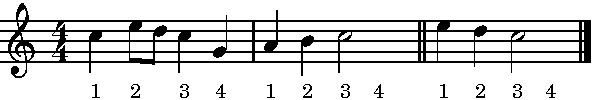
\includegraphics[width=0.8\linewidth]{me-temps.cropped.pdf}
\vfill
{\small\color{mygray}
Gravures LilyPond, composition \LaTeX.\\
Fichier MusicXML joint.\par}
\vspace{1cm}
\end{titlepage}

\tableofcontents
\newpage

% =====================================================================
\section{Avant-propos}

La \textbf{mesure} organise le temps de la musique : elle groupe des temps
égaux par deux, par trois ou par quatre, et appuie le premier de chaque groupe.
Le mot désigne aussi chacun de ces groupes, tel que les barres de mesure le
découpent sur la portée. Au début du morceau, le chiffre indicateur dit comment
la mesure est faite.

À lire après
\href{https://www.slashbin.net/musique/theorie/valeurs.pdf}{\emph{Les
valeurs}}, qui présentent les figures de notes et de silences, le point, la
liaison et les groupes irréguliers. Les exemples sont en clé de sol, que
présente
\href{https://www.slashbin.net/musique/theorie/lecture.pdf}{\emph{Lire les
notes}}.
Au programme de matières théoriques de l'École de musique Vincent-d'Indy, ces
notions relèvent des niveaux 1 à 6.

\begin{remarque}
\textbf{Conventions.} Les chiffres indicateurs s'écrivent ici sur une ligne,
3/4, et se lisent «~trois-quatre~». Les durées se comptent en fractions de
ronde : la noire vaut un quart de ronde, la croche un huitième. Sous les
portées des exemples, les chiffres numérotent les temps.
\end{remarque}

Le fichier MusicXML joint fait entendre chaque exemple ; la
section~\ref{sec:musicxml} le présente.

% =====================================================================
\section{Le temps et la mesure}
\label{sec:temps}

\textbf{La pulsation.} Sous la plupart des musiques bat une pulsation
régulière, celle que marque le pied ou la main qui frappe. Chacun de ses
battements est un \emph{temps}. Les temps sont égaux ; une note en remplit un,
plusieurs, ou une fraction.

\textbf{Des temps groupés.} L'oreille ne les entend pas tous pareils : elle les
groupe par deux, par trois ou par quatre, et sent un appui au début de chaque
groupe. Ce groupe est la \emph{mesure}, cet appui le \emph{temps fort}
(section~\ref{sec:forts}). Compter «~un, deux, trois, un, deux, trois~»,
c'est compter les temps d'une mesure à trois temps.

\textbf{Les barres de mesure.} Sur la portée, un trait vertical précède chaque
temps fort : la \emph{barre de mesure}. Entre deux barres se trouve une mesure,
et toutes les mesures d'un passage contiennent la même durée. Une \emph{double
barre}, deux traits fins, sépare deux parties d'un morceau ; la \emph{barre
finale}, un trait fin et un trait épais, le termine.

\gravure{me-temps}{Trois mesures à quatre temps, les temps comptés dessous :
une barre simple, une double barre, la barre finale.}

% =====================================================================
\section{Les chiffres indicateurs}
\label{sec:chiffres}

\textbf{Deux chiffres superposés.} Au début du morceau, après la clé et
l'armure, le \emph{chiffre indicateur} dit comment la mesure est faite. Il ne
se répète pas : il vaut jusqu'à ce qu'un autre le remplace.

\textbf{Le chiffre du haut} compte les temps de la mesure : 2, 3 ou 4.
\textbf{Le chiffre du bas} nomme la figure qui vaut un temps, par le nombre
qu'il en faut pour une ronde : 1 pour la ronde, 2 pour la blanche, 4 pour la
noire, 8 pour la croche, 16 pour la double croche. À 3/4, la mesure compte
trois temps, et chaque temps vaut une noire, un quart de ronde. Cette lecture
vaut pour les mesures simples ; les mesures composées se lisent autrement
(section~\ref{sec:composees}).

\textbf{Le C et le C barré.} Deux chiffres s'écrivent souvent par un signe :
C pour 4/4, et C barré d'un trait vertical pour 2/2, dit aussi \emph{alla
breve}. Ce C n'est pas une initiale. Il vient de la notation du Moyen Âge, où
un cercle désignait la division ternaire, dite parfaite, et un demi-cercle la
division binaire, dite imparfaite.

\gravure{me-c}{4/4 écrit C, puis 2/2 écrit C barré.}

% =====================================================================
\section{Les mesures simples}
\label{sec:simples}

\textbf{Le temps binaire.} Dans une \emph{mesure simple}, chaque temps se
divise en deux : une noire en deux croches, une blanche en deux noires. Le
temps est dit \emph{binaire}. Il dure une figure sans point, que le chiffre du
bas peut nommer.

\textbf{Unité de temps, unité de mesure.} L'\emph{unité de temps} est la figure
qui dure un temps ; l'\emph{unité de mesure}, celle qui remplit la mesure à elle
seule. À 3/4, ce sont la noire et la blanche pointée.

\tableau{mesure-simples}

\gravure{me-simples}{Les cinq mesures simples les plus courantes, chaque temps
rempli par son unité de temps.}

\textbf{Quatre noires ou deux blanches.} 4/4 et 2/2 contiennent la même durée,
une ronde, mais ne se comptent pas pareil : quatre temps à la noire, ou deux à
la blanche. Le 2/2 convient aux mouvements vifs, où l'on sent deux appuis plutôt
que quatre. D'autres mesures simples existent, plus rares : 3/2, fréquente dans
la musique baroque, ou 2/8.

\begin{remarque}
\textbf{Le 3/8.} Le 3/8 est une mesure simple à trois temps, la croche pour
unité de temps. Dans un mouvement rapide, pourtant, on le bat à un temps : ses
trois croches s'entendent comme la division d'une noire pointée, et la mesure
se comporte comme une mesure composée d'un seul temps --- certains auteurs la
rangent ainsi. Le chiffre ne change pas ; c'est le mouvement qui décide de la
battue.
\end{remarque}

% =====================================================================
\section{Temps forts et temps faibles}
\label{sec:forts}

\textbf{Le premier temps est fort.} Le premier temps de chaque mesure est le
\emph{temps fort} ; les autres sont des \emph{temps faibles}. Dans une mesure à
quatre temps, le troisième reçoit un appui moindre, mais réel : on le dit
\emph{mi-fort}, ou relativement fort.

\gravure{me-forts}{La force des temps, à deux, trois et quatre temps.}

Cet appui n'est pas forcément un son plus fort. C'est une attente de l'oreille,
que la mélodie et l'harmonie confirment d'ordinaire : les accords changent
volontiers sur le temps fort, et les phrases y aboutissent.

\textbf{Les parties du temps.} La même hiérarchie se répète à l'intérieur de
chaque temps. Divisé en deux, un temps a une \emph{partie forte}, la première
croche à 2/4, et une \emph{partie faible}, la seconde. Une partie faible est
plus faible que le temps qui la suit : la seconde croche d'un temps mène au
temps suivant.

\textbf{La battue.} Le chef d'orchestre, comme le musicien qui solfie, marque
les temps d'un geste de la main droite : c'est la \emph{battue}. Le premier
temps se bat toujours vers le bas, le dernier toujours vers le haut. À deux
temps : en bas, en haut. À trois temps : en bas, à droite, en haut. À quatre
temps : en bas, à gauche, à droite, en haut.

\textbf{L'anacrouse.} Une mélodie ne commence pas toujours sur un temps fort.
Les notes qui précèdent le premier temps fort forment l'\emph{anacrouse} : la
première mesure est incomplète, et la dernière lui rend d'ordinaire ce qui lui
manque, si bien qu'à elles deux elles font une mesure.

\gravure{me-anacrouse}{Une mélodie à 3/4 commencée sur le troisième temps :
une noire d'anacrouse, et une dernière mesure de deux temps.}

% =====================================================================
\section{Les mesures composées}
\label{sec:composees}

\textbf{Le temps ternaire.} Dans une \emph{mesure composée}, chaque temps se
divise en trois. Aucune figure sans point ne vaut trois croches : l'unité de
temps est une figure pointée, le plus souvent la noire pointée. Le temps est dit
\emph{ternaire}.

\textbf{Le chiffre compte les divisions.} Faute de chiffre pour une noire
pointée, le chiffre indicateur ne peut pas nommer l'unité de temps. Il compte
donc les divisions du temps : en haut, leur nombre dans la mesure ; en bas, leur
figure. À 6/8, la mesure contient six croches, groupées en deux temps de trois.
Pour retrouver le nombre de temps, on divise le chiffre du haut par trois ; pour
retrouver l'unité de temps, on pointe la figure qui vaut deux divisions : deux
croches font une noire, trois croches une noire pointée. Un chiffre du haut de
6, 9 ou 12 signale ainsi une mesure composée, à deux, trois ou quatre temps.

\tableau{mesure-composees}

\gravure{me-composees}{6/8 et 9/8 en croches, groupées par temps ; 12/8 en
noires pointées, une par temps.}

Aucune figure ne vaut neuf croches : la mesure à 9/8 n'a pas d'unité de mesure,
et il faut lier une blanche pointée à une noire pointée pour la remplir. Les
temps forts et faibles suivent les règles des mesures simples : à 12/8, quatre
temps, dont le troisième mi-fort. Chaque temps a une partie forte, sa première
division, et deux parties faibles.

% =====================================================================
\section{Mesures simples et mesures composées}
\label{sec:correspondances}

\textbf{Même nombre de temps, autre division.} À chaque mesure simple
correspond une mesure composée qui a le même nombre de temps, mais des temps
ternaires : son unité de temps est l'unité de temps simple, pointée. 2/4 et
6/8 ont deux temps, une noire dans l'une, une noire pointée dans l'autre.

\textbf{Le calcul.} On passe d'une mesure simple à sa correspondante composée
en multipliant le chiffre du haut par 3 et celui du bas par 2 : 2/4 devient
6/8, 3/4 devient 9/8. On revient en divisant.

\tableau{mesure-correspondances}

Si leurs temps vont à la même allure, deux mesures correspondantes durent
autant. En valeurs écrites, pourtant, la mesure à 6/8 vaut une fois et demie la
mesure à 2/4 : trois croches par temps au lieu de deux.

\textbf{Le triolet et le duolet.} Une mesure simple emprunte la division
ternaire le temps d'un \emph{triolet}, trois croches dans le temps de deux. Une
mesure composée emprunte la division binaire par le \emph{duolet}, deux croches
dans le temps de trois. Les deux figures sont présentées dans \emph{Les
valeurs}.

\gravure{me-correspondances}{2/4 puis 6/8 : deux temps chacune, divisés en deux
puis en trois. Un triolet à 2/4 sonne comme une mesure à 6/8, un duolet à 6/8
comme une mesure à 2/4.}

% =====================================================================
\section{Syncope et contretemps}
\label{sec:syncope}

\textbf{La syncope.} Une \emph{syncope} est un son attaqué sur un temps faible,
ou sur la partie faible d'un temps, et prolongé sur le temps ou la partie de
temps plus fort qui suit. L'appui attendu n'est pas attaqué : la note tenue le
recouvre, et l'accent se déplace sur elle. La prolongation s'écrit par une
valeur longue, ou par une liaison quand elle franchit une barre de mesure.

\gravure{me-syncopes}{Trois syncopes à 4/4 : une noire sur la partie faible du
premier temps, une noire liée du quatrième temps au premier de la mesure
suivante, une blanche du deuxième temps au troisième.}

Une note prolongée d'un temps fort sur un temps faible n'est pas une syncope :
elle allonge l'appui au lieu de le déplacer.

\textbf{Le contretemps.} Un \emph{contretemps} est un son attaqué sur un temps
faible, ou sur la partie faible d'un temps, après un silence placé sur le temps
ou la partie plus forte. L'appui tombe sur le silence ; la note arrive juste
après.

\gravure{me-contretemps}{Quatre contretemps à 2/4 : trois croches après un
demi-soupir, une noire après un soupir.}

La syncope tient la note par-dessus l'appui ; le contretemps laisse l'appui en
silence. Dans les deux cas, l'oreille entend l'appui quand même, et l'effet naît
de l'écart entre ce qu'elle attend et ce qu'elle entend.

% =====================================================================
\section{Les mesures irrégulières}
\label{sec:irregulieres}

\textbf{Des temps inégaux.} Certaines mesures n'ont ni des temps tous binaires,
ni des temps tous ternaires : 5/4, 5/8, 7/8\ldots{} Leurs temps sont inégaux.
Une mesure à 5/8 se bat en deux temps, l'un de deux croches, l'autre de trois ;
une mesure à 7/8 en trois temps, de deux, deux et trois croches, ou dans un
autre ordre. À 5/4, dans un mouvement modéré, on compte cinq noires, groupées
par trois et deux ou par deux et trois.

\textbf{Le groupement s'écrit.} Les poutres et les accents montrent le
groupement ; le chiffre indicateur l'écrit parfois en toutes lettres, 2+2+3
au-dessus de 8. On dit aussi ces mesures \emph{asymétriques}.
L'ethnomusicologue Constantin Brăiloiu a nommé \emph{aksak}, «~boiteux~» en
turc, les rythmes qui les emploient dans les musiques populaires des Balkans et
de Turquie.

\gravure{me-irregulieres}{Une mesure à 5/4 groupée par trois et deux noires,
puis deux mesures à 7/8, groupées par deux, deux et trois croches, puis par
trois, deux et deux. Un accent marque le début de chaque groupe.}

\textbf{Où on les trouve.} Le deuxième mouvement de la Sixième Symphonie de
Tchaïkovski, dite «~Pathétique~», est à 5/4, comme \emph{Mars}, qui ouvre
\emph{Les Planètes} de Holst. Bartók en fait la matière des \emph{Six danses en
rythme bulgare} qui terminent le \emph{Mikrokosmos}. Le jazz en a tiré un
succès avec \emph{Take Five}, à 5/4, de Paul Desmond pour le quartette de Dave
Brubeck.

% =====================================================================
% Une page à part : sans ce saut, les gravures des exercices passaient à la
% page suivante, loin de leur consigne.
\clearpage
\section{S'exercer}
\label{sec:exercices}

\textbf{Les chiffres.} Pour chacun des chiffres indicateurs suivants, dire si
la mesure est simple ou composée, combien elle a de temps, et quelle figure vaut
un temps : %% Produit par outils/generer_mesure.py — ne pas modifier à la main.
3/4, 6/8, 2/2, 12/8, 9/8, 4/4, 6/4 et 2/4
\unskip.

\textbf{Les mesures.} Les mesures ci-dessous ont perdu leur chiffre
indicateur. Le retrouver pour chacune, parmi
%% Produit par outils/generer_mesure.py — ne pas modifier à la main.
2/4, 3/4, 4/4, 3/8, 6/8, 9/8 et 12/8
\unskip. La durée de la mesure en
écarte la plupart ; les poutres et les valeurs longues départagent les autres.

\gravure{me-exercice-mesures}{Neuf mesures sans chiffre indicateur.}

\textbf{Syncopes et contretemps.} Pour chaque note numérotée, dire si elle
forme une syncope, un contretemps, ou ni l'un ni l'autre.

\gravure{me-exercice-syncopes}{À 4/4.}

\begin{remarque}
\textbf{Réponses.}

%% Produit par outils/generer_mesure.py — ne pas modifier à la main.
\textbf{Les chiffres.} 3/4~:~simple, trois temps, la noire~; 6/8~:~composée, deux temps, la noire pointée~; 2/2~:~simple, deux temps, la blanche~; 12/8~:~composée, quatre temps, la noire pointée~; 9/8~:~composée, trois temps, la noire pointée~; 4/4~:~simple, quatre temps, la noire~; 6/4~:~composée, deux temps, la blanche pointée~; 2/4~:~simple, deux temps, la noire.

\textbf{Les mesures.} 1~:~6/8~; 2~:~3/4~; 3~:~2/4~; 4~:~9/8~; 5~:~4/4~; 6~:~12/8~; 7~:~3/4~; 8~:~6/8~; 9~:~3/8.

\textbf{Syncopes et contretemps.} 1~:~ni l'un ni l'autre~; 2~:~syncope~; 3~:~contretemps~; 4~:~ni l'un ni l'autre~; 5~:~syncope~; 6~:~contretemps~; 7~:~contretemps~; 8~:~syncope.

\end{remarque}

% =====================================================================
\section{Le fichier MusicXML}
\label{sec:musicxml}

Le fichier joint, \texttt{mesure.musicxml}, reprend les exemples dans l'ordre
du guide, puis les deux exercices gravés, à la noire 80. Les chiffres
indicateurs y figurent : il donne aussi les réponses de l'exercice des mesures.
Il se lit avec MuseScore, Finale, Sibelius, Dorico ou tout éditeur de
partitions ; sur slashbin.net, il s'écoute aussi dans Sodor Piano.

% =====================================================================
\section*{Colophon}
\addcontentsline{toc}{section}{Colophon}

Les gravures musicales sont produites par \textbf{LilyPond}, la composition
par \textbf{\LaTeX}. Les tableaux, les mots placés sous les temps et au-dessus
des notes, les réponses des exercices et le fichier MusicXML dérivent d'une
seule donnée par mesure, son chiffre indicateur, dont le générateur déduit le
genre de la mesure, ses temps et ses unités, et la force de chaque temps et de
chaque partie de temps. Avant d'écrire quoi que ce soit, il vérifie ce que le
texte affirme : les unités de chaque mesure, les correspondances entre mesures
simples et composées, chaque mesure complète, les syncopes et les contretemps
des exemples, et le chiffre unique de chaque mesure de l'exercice. Pour
régénérer l'ensemble :

\begin{center}
\texttt{python3 outils/generer\_mesure.py}\\
\texttt{(cd gravures \&\& lilypond -dcrop --formats=pdf me-*.ly)}\\
\texttt{pdflatex mesure.tex}
\end{center}

\end{document}
